\documentclass[12pt,final,twoside]{report}
%%%%%%%%%%%%%%%%%%%%%%%%%%%%%%%%%%%%%%%%%%%%%%%%%%%%%%%%%%%%%
% Some credits:
% The template initially was created by Prof. Dr. Holger Karl/Uni Paderborn '2006
% and was expanded and updated by 
% - Stefan Heinrich/Uni Paderborn/Uni Hamburg since 2008,
% - Sven Magg/Uni Hamburg since 2013.
% Suggestions for changes are always welcome.
%%%%%%%%%%%%%%%%%%%%%%%%%%%%%%%%%%%%%%%%%%%%%%%%%%%%%%%%%%%%%
% Meta information:
\newcommand{\trtitle}{Compositional Generalization in Transformers}
\newcommand{\trtype}{Masterthesis} %{Bachelorthesis} %{Diplomarbeit} %{Dissertation}
\newcommand{\trcourseofstudies}{Intelligent Adaptive Systems} %{Bioinformatik} %{Intelligent Adaptive Systems} 
\newcommand{\trauthor}{Imran Ibrahimli}
\newcommand{\trauthordegree}{} %{\ B.Sc.}
\newcommand{\tremail}{imran.ibrahimli@studium.uni-hamburg.de}
\newcommand{\trmatrikelnummer}{7486484}
\newcommand{\trgutachterA}{\href{mailto:stefan.wermter@uni-hamburg.de}{Prof. Dr. Stefan Wermter}}
\newcommand{\trgutachterB}{\href{mailto:jae.hee.lee@uni-hamburg.de}{Dr. Jae Hee Lee}}
%\newcommand{\trbetreuung}{\href{mailto:tbd@informatik.uni-hamburg.de}{Dipl.-Inform. To Be Defined}}
\newcommand{\trfach}{Knowledge Technology, WTM}
\newcommand{\trdate}{24.10.2024}
\newcommand{\trkeywords}{Transformer, Algorithms, Mechanistic Interpretability}
%Optionally: it is also allowed to provide a street name on the
%\newcommand{\trstrasse}{Streetname 42}
%\newcommand{\trort}{22527 Hamburg}

%%%%%%%%%%%%%%%%%%%%%%%%%%%%%%%%%%%%%%%%%%%%%%%%%%%%%%%%%%%%%
% Languages:

% Falls die Ausarbeitung in Deutsch erfolgt:
% \usepackage[german]{babel}
% \usepackage[T1]{fontenc}
% \usepackage[latin1]{inputenc}
% \usepackage[latin9]{inputenc}                     
% \selectlanguage{german}

% If the thesis is written in English:
\usepackage[english]{babel}                         
\selectlanguage{english}

%%%%%%%%%%%%%%%%%%%%%%%%%%%%%%%%%%%%%%%%%%%%%%%%%%%%%%%%%%%%%
% Bind packages:
\usepackage{acronym}                    % Acronyms
\usepackage{algorithmic}                % Algorithms and Pseudocode
\usepackage{algorithm}                  % Algorithms and Pseudocode
\usepackage{amsfonts}                   % AMS Math Packet (Fonts)
\usepackage{amsmath}                    % AMS Math Packet
\usepackage{amssymb}                    % Additional mathematical symbols
\usepackage{amsthm}
\usepackage{booktabs}                   % Nicer tables
%\usepackage[font=small,labelfont=bf]{caption} % Numbered captions for figures
\usepackage{color}                      % Enables defining of colours via \definecolor
\definecolor{uhhRed}{RGB}{226,0,26}     % Official Uni Hamburg Red
\definecolor{uhhGrey}{RGB}{136,136,136} % Official Uni Hamburg Grey
\definecolor{uhhLightGrey}{RGB}{220, 220, 220}
\usepackage{fancybox}                   % Put equations in a frame
\usepackage{fancyhdr}                   % Packet for nicer headers
%\usepackage{fancyheadings}             % Nicer numbering of headlines
\usepackage[body={5.8in,9in}]{geometry} % Type area (size, margins...)

%\geometry{a4paper,outer=3.35cm}        % !!!Release version (Normal margins)
%\geometry{a4paper,outer=2.5cm}         % !!!Print version (Additional margin on the left for the binding)
%\geometry{a4paper}                     % !!!Proofread version (Additional margin on the right for corrections)
\geometry{a4paper,outer=3.134cm}        % !!!Draft version (Same margins on left and right)
%\geometry{paperheight=10.0in,paperwidth=6.4in,top=0.51in,left=0.3in}  % !!!Developer version (Minimal margins)

\usepackage{graphicx}                   % Inclusion of graphics
%\usepackage{latexsym}                  % Special symbols
\usepackage{longtable}                  % Allow tables over several parges
\usepackage{listings}                   % Nicer source code listings
\usepackage{multicol}                   % Content of a table over several columns
\usepackage{multirow}                   % Content of a table over several rows
\usepackage{rotating}                   % Alows to rotate text and objects
%\usepackage{siunitx}					% Nicer display of units and number according to SI standards
%\sisetup{tight-spacing=true}  
\usepackage[hang]{subfigure}            % Allows to use multiple (partial) figures in a fig
%HINT: subfigure may be depricated already - maybe try subfig instead 
%\usepackage[font=footnotesize,labelfont=rm]{subfig}    % Pictures in a floating environment
\usepackage{tabularx}                   % Tables with fixed width but variable rows
\usepackage{url,xspace,boxedminipage}   % Accurate display of URLs

%%%%%%%%%%%%%%%%%%%%%%%%%%%%%%%%%%%%%%%%%%%%%%%%%%%%%%%%%%%%%
% PDF Information und Definitions:
\author{\trauthor}

\ifx\pdftexversion\undefined
\usepackage{hyperref}
\else
\usepackage[colorlinks=false,           % link is colores (true) or has colored frame (false)
            linkcolor=uhhRed,           % case colorlinks=true: define color.
            urlcolor=uhhRed,
            citecolor=uhhRed,
            bookmarks,                  % Place bookmarks erstellen
            bookmarksopen=true,         % Bookmarks will be shown at start (true/false)
            pdfpagemode=UseOutlines,    
            bookmarksopenlevel=1,       % Define the depth of shown links
            bookmarksnumbered,          % Numbers of chapers in Bookmarks
            pdftitle={\trtitle},
            pdfsubject={\trtype},
            pdfkeywords={\trkeywords},
            pdfauthor={\trauthor},
            plainpages=false
            ]{hyperref}
\fi

\ifx\pdftexversion\undefined
\else
\pdfoutput=1                            % Disable PDF-Output
\pdfimageresolution=1200
\pdfcompresslevel=2                     % 0 = no compression, 9 = strongest compression
\fi

%%%%%%%%%%%%%%%%%%%%%%%%%%%%%%%%%%%%%%%%%%%%%%%%%%%%%%%%%%%%%
% Configurationen:

\hyphenation{whe-ther}                  % Manually use: "\-" in a word: Staats\-ver\-trag

%\lstloadlanguages{C}                   % Set the default language for listings
\DeclareGraphicsExtensions{.pdf,.svg,.jpg,.png,.eps} % first try pdf, then eps, png and jpg
\graphicspath{{./img/}}                 % Path to a folder where all pictures are located
\pagestyle{fancy}                       % Use nicer header and footer

% Redefine the environments for floating objects:
\setcounter{topnumber}{3}
\setcounter{bottomnumber}{2}
\setcounter{totalnumber}{4}
\renewcommand{\topfraction}{0.9}        %Standard: 0.7
\renewcommand{\bottomfraction}{0.5}     %Standard: 0.3
\renewcommand{\textfraction}{0.1}       %Standard: 0.2
\renewcommand{\floatpagefraction}{0.8}  %Standard: 0.5

% Tables with a nicer padding:
\renewcommand{\arraystretch}{1.2}

% Chapter and Sections will not be written in capitals
\renewcommand{\chaptermark}[1]{\markboth{\chaptername \ \thechapter.\ #1}{}}
\renewcommand{\sectionmark}[1]{\markright{\thesection.\ #1}}

% Avoid french spacing (double spacing after a full stop)
\frenchspacing

%%%%%%%%%%%%%%%%%%%%%%%%%%%%
% Additional 'theorem' and 'definition' blocks:
\theoremstyle{plain}
\newtheorem{theorem}{Theorem}[chapter]
%\newtheorem{theorem}{Satz}[chapter]    % Wenn in Deutsch geschrieben wird.
\newtheorem{axiom}{Axiom}[chapter]     
%\newtheorem{axiom}{Fakt}[chapter]      % Wenn in Deutsch geschrieben wird.
%Usage:%\begin{axiom}[optional description]%Main part%\end{fakt}

\theoremstyle{definition}
\newtheorem{definition}{Definition}[chapter]

%Additional types of axioms:
\newtheorem{lemma}[axiom]{Lemma}
\newtheorem{observation}[axiom]{Observation}

%Additional types of definitions:
\theoremstyle{remark}
%\newtheorem{remark}[definition]{Bemerkung} % Wenn in Deutsch geschrieben wird.
\newtheorem{remark}[definition]{Remark} 

%%%%%%%%%%%%%%%%%%%%%%%%%%%%
% Provides TODOs within the margin:
\newcommand{\TODO}[1]{\marginpar{\emph{\small{{\bf TODO: } #1}}}}

%%%%%%%%%%%%%%%%%%%%%%%%%%%%
% Abbreviations and mathematical symbols
\newcommand{\modd}{\text{ mod }}
\newcommand{\RS}{\mathbb{R}}
\newcommand{\NS}{\mathbb{N}}
\newcommand{\ZS}{\mathbb{Z}}
\newcommand{\dnormal}{\mathit{N}}
\newcommand{\duniform}{\mathit{U}}

\newcommand{\erdos}{Erd\H{o}s}
\newcommand{\renyi}{-R\'{e}nyi}
% it is recommented to define complex terms as expression/newcommand and use the expression in the tex instead.

%%%%%%%%%%%%%%%%%%%%%%%%%%%%%%%%%%%%%%%%%%%%%%%%%%%%%%%%%%%%%
% Document:

\begin{document}

\pagenumbering{Roman}                   % Roman pagenumbering for lists and meta pages
\renewcommand{\headheight}{14.5pt}      % Size of headings

\thispagestyle{empty}
\fancyhead[LO,RE]{}                     % Define the header style for the meta pages

%%%%%%%%%%%%%%%%%%%%%%%%%%%%
% Cover sheet

\begin{titlepage}
  %---Possibility 1:
  \begin{flushleft}
    
\includegraphics[width=67mm]{uhhLogoL.pdf}\\
  \end{flushleft}
  \rule{\textwidth}{0.4pt}
  \newline
  \vspace{2.0cm}
  \begin{center}
    \LARGE \textbf{\trtitle}
  \end{center}
  \vspace{2.0cm}
  \begin{center}
    \textbf{\trtype}\\
    %im Arbeitsbereich \trfach\\
    at Research Group \trfach\\
    \trgutachterA\medskip\\
    %Fachbereich Informatik\\
    Department of Informatics\\
    %MIN-Fakult\"at\\
    MIN-Faculty\\
    Universit\"at Hamburg \\[1.0cm] %not allowed to translate Universit{\"a}t Hamburg
    %vorgelegt von \\
    submitted by \\
    \textbf{\href{mailto:\tremail}{\trauthor\trauthordegree}}\\
    %Studiengang:   \trcourseofstudies \\
    Course of study:   \trcourseofstudies \\
    Matrikelnr.:  \trmatrikelnummer \\
    %a\\
    on\\
    \trdate
  \end{center}
  \vspace{2cm}
  \begin{center}
    \begin{tabular}{ll}
      %Gutachter: & \trgutachterA \\
      Examiners: & \trgutachterA \\
                 & \trgutachterB \\
      %Betreuung: & \trbetreuung \\    	% Adviser are not allowed to demand getting mentioned here, but are happy getting credited by student's initiative
    \end{tabular}
  \end{center}
  \vfill
  %    \begin{tabular}{l}
  %    \trauthor \\
  %    Matrikelnummer:  \trmatrikelnummer \\
  %    \trstrasse \\
  %    \trort
  %    \end{tabular}
  %    \newline
  \rule{\textwidth}{0.4pt}
  \newpage
\end{titlepage}

%backsite of cover sheet is empty!
\thispagestyle{empty}
\hspace{1cm}
\newpage

%%%%%%%%%%%%%%%%%%%%%%%%%%%%
% Abstract:
\section*{Abstract}\label{sec:abstract}
%\fancyhead[LE,RO]{\it Abstract}
%\addcontentsline{toc}{chapter}{\numberline{}Abstract}
Your English abstract here (mandatory if written in English and recommended otherwise).

% If the abstract ist not longer than half a page, then the German Zusammenfassung can be places on the same page
%\cleardoublepage
\vfill
\section*{Zusammenfassung}\label{sec:zusammenfassung}
%\addcontentsline{toc}{chapter}{\numberline{}Zusammenfassung} %Add the Zusammenfassung to the TOC
Hier die deutsche Zusammenfassung einf\"ugen (notwendig).
\fancyhead[LE,RO]{\it Abstract}

\cleardoublepage

%%%%%%%%%%%%%%%%%%%%%%%%%%%%
% Lists:
%\setcounter{tocdepth}{1}               % depth of the table of contents (for BSc and MSc Thesis 1 is recommented)
\fancyhead[LE,RO]{\it Contents}
\tableofcontents
\cleardoublepage
% List of Figures and List of tables are optional. -> Not needed in most theses.
\fancyhead[LE,RO]{\it List of Figures}
\listoffigures
\cleardoublepage
\fancyhead[LE,RO]{\it List of Tables}
\listoftables
\cleardoublepage
%\lstlistoflistings
%\cleardoublepage

\fancyhead[LE]{\it \leftmark}           % Define the header style for the text pages
\fancyhead[RO]{\it \rightmark}          % Define the header style for the text pages
\fancyhead[LO,RE]{}                     % Define the header style for the text pages

%%%%%%%%%%%%%%%%%%%%%%%%%%%%
% The content will be included here:
\pagenumbering{arabic}

\chapter{Introduction}\label{introduction}



An Introduction usually is used only to provide a background, a motivation and a short readers guide. In this document it is used to reproduce some information about writing a thesis and writing in \LaTeX. To get started, just delete this content and start writing your own.

\section{How to Organize your Thesis}
In this section some revision of a generic structure of a thesis will be given. Please note that the complete text can be found on:
\begin{quote}
	http://www.sce.carleton.ca/faculty/chinneck/thesis.html
\end{quote}
Translations to other languages are available too:
\begin{quote}
	http://www.sce.carleton.ca/faculty/chinneck/thesis/translations.html
\end{quote}


\subsection{Introduction}

This is a general introduction to what the thesis is all about -- it is not just a description of the contents of each section. Briefly summarize the question (you will be stating the question in detail later), some of the reasons why it is a worthwhile question, and perhaps give an overview of your main results. This is a birds-eye view of the answers to the main questions answered in the thesis (see above).

\subsection{Background Information (optional)}

A brief section giving background information may be necessary, especially if your work spans two or more traditional fields. That means that your readers may not have any experience with some of the material needed to follow your thesis, so you need to give it to them. A different title than that given above is usually better; e.g., 'A Brief Review of Frammis Algebra.'

\subsection{Review of the State of the Art}

Here you review the state of the art relevant to your thesis. Again, a different title is probably appropriate; e.g., 'State of the Art in Zylon Algorithms.' The idea is to present (critical analysis comes a little bit later) the major ideas in the state of the art right up to, but not including, your own personal brilliant ideas.

You organize this section by idea, and not by author or by publication. For example if there have been three important main approaches to Zylon Algorithms to date, you might organize subsections around these three approaches, if necessary:
\begin{itemize}
	\item[3.1] Iterative Approximation of Zylons
	\item[3.2] Statistical Weighting of Zylons
	\item[3.3] Graph-Theoretic Approaches to Zylon Manipulation
\end{itemize}

\subsection{Research Question or Problem Statement}

Engineering theses tend to refer to a 'problem' to be solved where other disciplines talk in terms of a 'question' to be answered. In either case, this section has three main parts:

\begin{enumerate}
	\item a concise statement of the question that your thesis tackles
	\item justification, by direct reference to section 3, that your question is previously unanswered
	\item discussion of why it is worthwhile to answer this question.
\end{enumerate}

Item 2 above is where you analyze the information which you presented in Section 3. For example, maybe your problem is to 'develop a Zylon algorithm capable of handling very large scale problems in reasonable time' (you would further describe what you mean by 'large scale' and 'reasonable time' in the problem statement). Now in your analysis of the state of the art you would show how each class of current approaches fails (i.e. can handle only small problems, or takes too much time). In the last part of this section you would explain why having a large-scale fast Zylon algorithm is useful; e.g., by describing applications where it can be used.

Since this is one of the sections that the readers are definitely looking for, highlight it by using the word 'problem' or 'question' in the title: e.g. 'Research Question' or 'Problem Statement', or maybe something more specific such as 'The Large-Scale Zylon Algorithm Problem.'

\subsection{Description of How You Solved the Problem or Answered the Question}

This part of the thesis is much more free-form. It may have one or several sections and subsections. But it all has only one purpose: to convince the examiners that you answered the question or solved the problem that you set for yourself in Section 4. So show what you did that is relevant to answering the question or solving the problem: if there were blind alleys and dead ends, do not include these, unless specifically relevant to the demonstration that you answered the thesis question.

\subsection{Conclusions}

You generally cover three things in the Conclusions section, and each of these usually merits a separate subsection:

\begin{enumerate}
	\item Conclusions
	\item Summary of Contributions
	\item Future Research
\end{enumerate}

Conclusions are not a rambling summary of the thesis: they are short, concise statements of the inferences that you have made because of your work. It helps to organize these as short numbered paragraphs, ordered from most to least important. All conclusions should be directly related to the research question stated in Section 4. Examples:

\begin{enumerate}
	\item The problem stated in Section 4 has been solved: as shown in Sections ? to ??, an algorithm capable of handling large-scale Zylon problems in reasonable time has been developed.
	\item The principal mechanism needed in the improved Zylon algorithm is the Grooty mechanism.
	\item Etc.
\end{enumerate}

The Summary of Contributions will be much sought and carefully read by the examiners. Here you list the contributions of new knowledge that your thesis makes. Of course, the thesis itself must substantiate any claims made here. There is often some overlap with the Conclusions, but that's okay. Concise numbered paragraphs are again best. Organize from most to least important. Examples:

\begin{enumerate}
	\item Developed a much quicker algorithm for large-scale Zylon problems.
	\item Demonstrated the first use of the Grooty mechanism for Zylon calculations.
	\item Etc.
\end{enumerate}

The Future Research subsection is included so that researchers picking up this work in future have the benefit of the ideas that you generated while you were working on the project. Again, concise numbered paragraphs are usually best. 

\subsection{Appendices}

What goes in the appendices? Any material which impedes the smooth development of your presentation, but which is important to justify the results of a thesis. Generally it is material that is of too nitty-gritty a level of detail for inclusion in the main body of the thesis, but which should be available for perusal by the examiners to convince them sufficiently. Examples include program listings, immense tables of data, lengthy mathematical proofs or derivations, etc. 

\subsection{Bibliography}

The list of references is closely tied to the review of the state of the art given in section 3. Most examiners scan your list of references looking for the important works in the field, so make sure they are listed and referred to in section 3. Truth be known, most examiners also look for their own publications if they are in the topic area of the thesis, so list these too. Besides, reading your examiner's papers usually gives you a clue as to the type of questions they are likely to ask.

All references given must be referred to in the main body of the thesis. Note the difference from a Bibliography, which may include works that are not directly referenced in the thesis. Organize the list of references either alphabetically by author surname (preferred), or by order of citation in the thesis. 



\section{Revision: Writing in \LaTeX}
As thought in the seminars, \LaTeX is quite useful for writing a paper or a thesis. Nevertheless it comes with its own rules.

\subsection{Word processing with \LaTeX}
\label{sec:model:subsec:latex}

This document has already introduced the most important constructs of
\LaTeX. What is necessary to produce documents with \LaTeX is simple
any normal text editor and a \LaTeX distribution. This is commonly
installed on practically all UNIX-type systems; for Windows, an
excellent \LaTeX exists, called MikTeX, available from
\url{www.miktex.org}. Almost all distributions come with a large patch
of examples and introductory material; consult your local installation
for details. 

Lots of supplementary and background information, FAQs, etc.\ is
available from the Comprehensive TeX Archive Network (CTAN); the
German mirror of which is \url{www.dante.de}. 

\subsection{Tables in \LaTeX}
\label{sec:model:subsec:tables}
The table should be centred and should always have a caption positioned above it. A caption in a sentence form as well as in a short form must end with a period as seen in table~\ref{tab:sample}. Ideally the table can be understood sorely by the table and the caption itself. The parameters ``hbtp'' provide a list of priorities for the arrangement of the table: here, bottom, top, (next) page.

\begin{table}[hbtp]
	\caption{This caption has one line so it is centered.}\label{tab:sample}
	\centering
	\begin{tabular}{|c|c|}
		\hline
		Example column 1 & Example column 2 \\
		\hline
		Example text 1   & Example text 2   \\
		\hline
	\end{tabular}
\end{table}

\subsection{Figures in \LaTeX}
\label{sec:model:subsec:figures}
Note that a figure is a so-called floating object: it is moved around the actual text in order to best fit on a page. This is in strong contrast to some GUI-based word processing tools, where the placement of figures is usually more associated with luck than principle.

As figures float around, expressions like ``the following figure'' must never be used. Instead, figures need a caption, a label, and must be properly referenced in the main text. A figure caption is placed centred below the figure and describes the figure in (very) short. Again, ideally the figure can be understood sorely by the figure and the caption itself.

In general, only vector graphics in encapsulated postscript (EPS) or a similar format (SVG, PDF) should be included in any kind of text, as this allows arbitrary scaling, rotation etc.\ without any loss of quality. Bitmap formats (JPEG, GIF, \dots) should only be used if no other alternative exists --- basically the only case where bitmaps can be justified is when scanned pictures need to be included in a text, however, this should be avoided as hard as possible as the quality in usually not satisfactory. If a screen shot is needed a high resolution picture without visible fragments of a jpeg compression is allowed. Figures like the figure~\ref{fig:samplefig} (this is how you refer to figures correctly! the tilde is used as a non-breaking space) should always appear after the first referencing it.
\begin{figure}[hbtp]
	\centerline{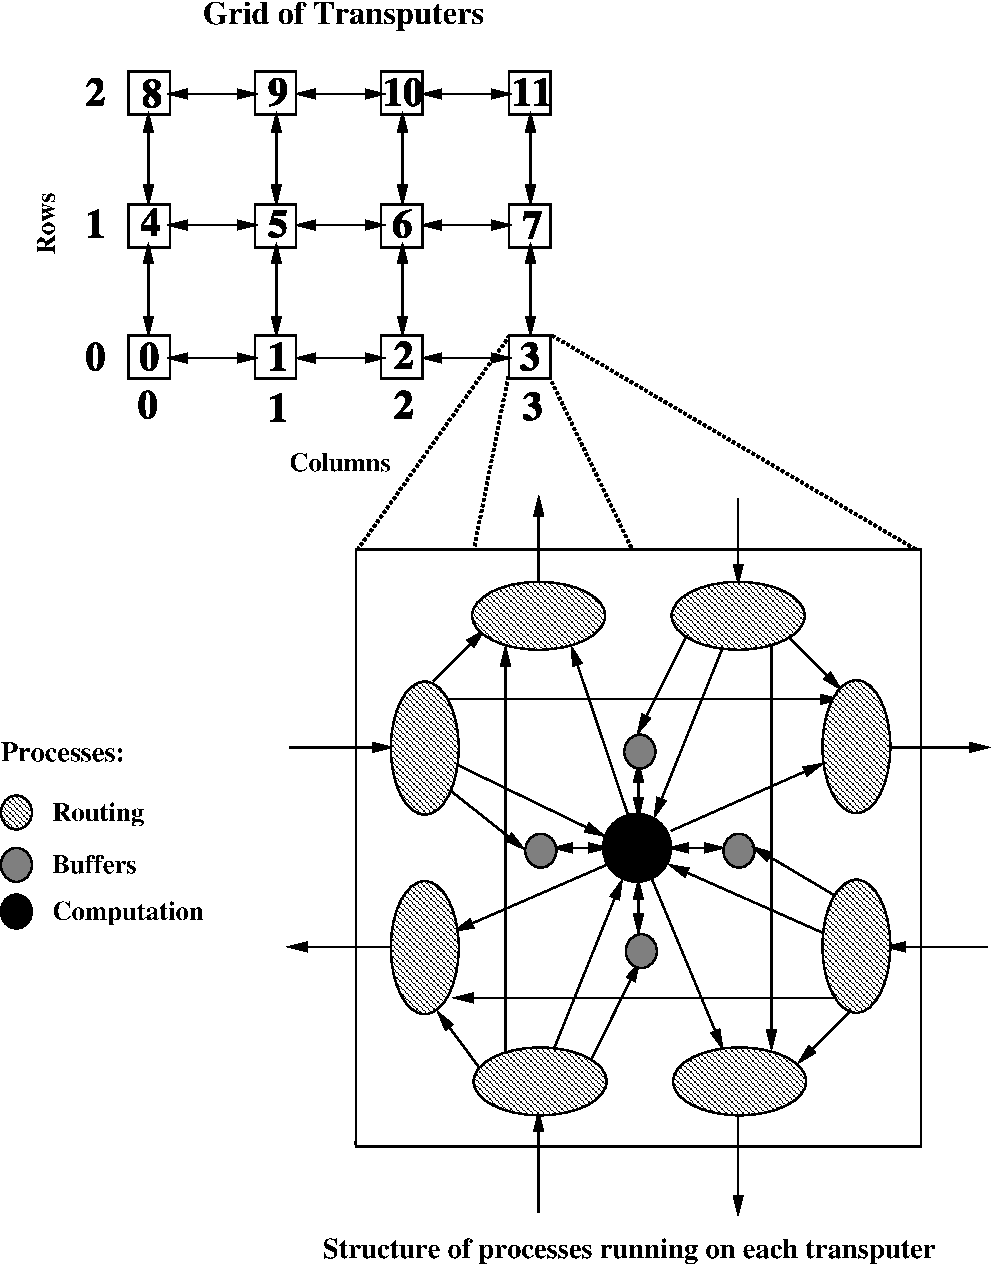
\includegraphics[width=0.6\textwidth]{samplefig.pdf}}
	{\caption{Network of transputers and the structure of individual
			processes.}\label{fig:samplefig}}
\end{figure}
\cleardoublepage

\chapter{Basics}\label{basics}

\section*{Research Questions: (TODO: ask Jae)}

\begin{enumerate}
    \item How do (smaller) transformers learn to compose sub-tasks for integer addition?
    \item What architectural features or training strategies enhance compositional learning?
    \item Do these models generalize to larger sequences than seen during training?
\end{enumerate}

Compositionality gap: difference between performance on subtasks and the full task. In our case full task is integer addition, with subtasks being digit-wise alignment, addition, and carry operations.

\subsection*{Experiments / Hypotheses (Baseline)}

\begin{itemize}
    \item RQ3: Models generalize to in-distribution sequence lengths but not OOD (longer or shorter) lengths.
          \begin{itemize}
              \item Baseline performance.
              \item Smaller $3 \times 3$, $7 \times 7$ experiments, 1-19 digits and 18/20+ digits
              \item Scratchpad can improve it to 18 and 20, not 21+
          \end{itemize}

    \item RQ1: Sub-task decomposition: models decompose addition into:
          \begin{itemize}
              \item digit-wise alignment
              \item modular digit-wise addition
              \item carry operations
              \item Probing tasks for sub-task neural networks, saliency, etc. (TODO)
          \end{itemize}

    \item RQ2: Positional embeddings are important for digit-wise addition and source of errors (e.g., alignment).
          \begin{itemize}
              \item Random spaces
              \item Abacus
              \item Relative pos encodings
          \end{itemize}

    \item RQ1: Compositional learning strategies:
          \begin{itemize}
              \item Simple to complex tasks (curriculum)
              \item Multi-task learning (aux loss) (TODO)
          \end{itemize}

    \item Error analysis: TODO for robustness.

\end{itemize}

\cleardoublepage

\chapter{Approach}\label{approach}
\cleardoublepage

\chapter{Results}\label{results}
\cleardoublepage

\chapter{Conclusion}\label{conclusion}
\cleardoublepage

%%%%%%%%%%%%%%%%%%%%%%%%%%%%
% Appendices:
% these are optional! For most Bachelor-theses and some Master-thesis none of them is needed. 
% Just comment them if not needed.
\appendix
\fancyhead[LO,RE]{}                      % Define the header style for the appendixpages

\fancyhead[LE,RO]{\it Anhang A. Nomenclature}                %Adapt letter!
\chapter{Nomenclature}\label{app:nomenclature}

\cleardoublepage

% ... add as much appendices as you need (one can also add source code, for example)

%\fancyhead[LE]{\it \leftmark}
%\chapter{}
\fancyhead[LE,RO]{\it Bibliography}       % A bibliography never have a letter or numbering!
\bibliographystyle{plain}             % Style for presenting the literature
\phantomsection\addcontentsline{toc}{chapter}{Bibliography}% Add to the TOC
\bibliography{thesis}
\cleardoublepage

%%%%%%%%%%%%%%%%%%%%%%%%%%%%
% Formal page 1
\vspace{2cm}
\chapter*{Erkl\"arung der Urheberschaft}
\label{sec:urheber}
\fancyhead[LE]{\it Erkl\"arung der Urheberschaft}
Hiermit versichere ich an Eides statt, dass ich die vorliegende
\trtype{} im Studiengang \trcourseofstudies{}
selbstst{\"a}ndig verfasst und keine anderen als die angegebenen
Hilfsmittel - insbesondere keine im Quellenverzeichnis nicht
benannten Internet-Quellen – benutzt habe. Alle Stellen, die
w{\"o}rtlich oder sinngem{\"a}{\ss} aus Ver{\"o}ffentlichungen entnommen wurden,
sind als solche kenntlich gemacht. Ich versichere weiterhin, dass
ich die Arbeit vorher nicht in einem anderen Pr{\"u}fungsverfahren
eingereicht habe und die eingereichte schriftliche Fassung der
auf dem elektronischen Speichermedium entspricht.

\vspace{4cm}
\noindent Ort, Datum \hfill Unterschrift

%The backcover is always empty
\newpage
\thispagestyle{empty}
\hspace{1cm}
\newpage

%%%%%%%%%%%%%%%%%%%%%%%%%%%%
% Formal page 2
\vspace{2cm}
\chapter*{Erkl\"arung zur Ver\"offentlichung}
\label{sec:urheber}
\fancyhead[LE]{\it Erkl\"arung zur Ver\"offentlichung}
Ich stimme der Einstellung der \trtype{} in die Bibliothek des Fachbereichs Informatik zu.

\vspace{4cm}
\noindent Ort, Datum \hfill Unterschrift

%The backcover is always empty
\newpage
\thispagestyle{empty}
\hspace{1cm}
\newpage

\end{document}
%EOF

